So far, we have only considered robustness for continuous problems. Many real-world applications require discrete, i.e., integer or binary decisions. This chapter focuses on robust formulations for these problems.

\section{Robust Mixed Integer Optimization}

We consider the nominal MIO problem:
\begin{align*}
\min & c^Tx \\
\stnew & Ax\leq b , \\
& x_i\in\integers_+,\;\forall i\in [k],\; x_i\in\reals,\;\forall i\in[n]\setminus [k],
\end{align*}
with $c\in\reals^n$, $b\in\reals^m$ and $A\in\reals^{m\times n}$. As discussed in chapter \ref{chapter3-2}, the derivation of the RC also holds for integer variables $x$. Hence, these reformulations can also be used for robust MIO problems. We thus have the following reformulations for the uncertain constraint $(\ol{a}+Pz)^Tx\leq b$, $z\in\keyunc$:
\begin{center}
\begin{tabular}{|l|c|c|c|}
\hline
Set type & $\keyunc$ & RC & Tractability \\
\hline
Box & $\norm{z}_\infty\leq\rho$ & $\ol{a}^Tx+\rho\norm{P^Tx}_1\leq b$ & MIO \\
\hline
Ellipsoidal &  $\norm{z}_2\leq\rho$ & $\ol{a}^Tx+\rho\norm{P^Tx}_2\leq b$ & CQMIO \\
\hline
Budget &  
\begin{tabular}{@{}c@{}}$\norm{z}_\infty\leq\rho$ \\ $\norm{z}_1\leq\Gamma$\end{tabular}
&  $\ol{a}^Tx+\rho\norm{y}_1+\Gamma\norm{P^Tx-y}_\infty\leq b$ & MIO \\
\hline
 Polyhedral &  $d-Dz\geq 0$ & 
 \begin{tabular}{@{}c@{}}$\ol{a}^Tx+d^Tv\leq b$ \\ $D^Tv=P^Tx$ \\ $v\geq 0$ \end{tabular}
& MIO \\
\hline
\end{tabular}
\end{center}
However, the original problem structure is not preserved, for example, the RC of the knapsack problem wit budget uncertainty is not a knapsack problem anymore. This means that problem-specific solution algorithms can no longer be applied.

\section{Robust Binary Optimization}

Examples of binary optimization problems include the shortest path, the minimum spanning tree, the traveling salesman and the vehicle routing problem. Surprisingly, if a binary optimization is solvable in polynomial time, so is its robust counterpart. More specifically, we consider problems of the form
\begin{align}\label{p3c4:binRO}
Z_R = & \min  && c^Tx + \max\limits_{S:\;S\subseteq[n],\vert S\vert\leq\Gamma} \sum\limits_{j\in S}d_jx_j \\
& \stnew && x\in\mathcal{F},
\end{align}
where $\mathcal{F}\subseteq \{0,1\}^n$ is the feasible set, and the coefficients $c_j\in[\ol{c}_j,\ol{c}_j+d_j]$ for $j\in[n]$ are uncertain,and at most $\Gamma$ of them are allowed to change. Without loss of generality, we assume that the indices are ordered such that $d_1\geq d_2\geq \dots\geq d_n$, and define $d_{n+1} = 0$ for notational convenience.

\begin{theorem}\label{p3c4:thm:n+1prob}
Problem \eqref{p3c4:binRO} reduces to solving n+1 nominal problems:
\[Z_R = \min\limits_{\ell\in [n+1]} G_\ell ,\]
where for $\ell \in [n+1]$:
\begin{align}\label{p3c4:G_l}
G_\ell = \Gamma d_\ell +\min\limits_{\ell\in [n+1]} & \big( c^Tx+\sum\limits_{j=1}^\ell (d_j-d_\ell)x_j\big) \\
& \stnew x\in\mathcal{F}.
\end{align}
\end{theorem}
This corresponds to solving $n+1$ problems of the same structure as the nominal problem.

\begin{proof}
Problem \eqref{p3c4:binRO} can be reformulated by introducing variables $u_j,j\in[n]$ indicating whether the coefficients $c_j,j\in[n]$ deviate in the worst case. We thus obtain
\begin{equation}
\begin{array}{rlll}
 Z_R = &\min\limits_ {x\in \mathcal{F}}&\left(c^Tx+\max\sum\limits_{j\in [n]}d_jx_ju_j\right) & \\
 					&\text{s.t. } &  \sum\limits_{j\in [n]}u_j\leq\Gamma & \text{(knapsack constraint)}\\
 							&  & u_j\in \{0,1\}, & \forall j\in [n] \\
\end{array}
\end{equation}
We can now relax the integrality constraint $u_j\in\{0,1\}$ to $0\leq u_j\leq 1$: In the knapsack constraint all $u_j$ have equal weight. The optimal solution thus assigns maximal value to $\Gamma$ variables $u_j$, namely the ones with the highest cost coefficients $d_jx_j$, and value $0$ to the others, so the optimal solution is guaranteed to be integer, provided that $\Gamma\in\integers_+$. Thus, we obtain
\begin{equation}
\begin{array}{rlll}
 Z_R = &\min\limits_ {x\in \mathcal{F}}&\left(c^Tx+\max\sum\limits_{j\in [n]}d_jx_ju_j\right) & \\
 					&\text{s.t. } &  \sum\limits_{j\in [n]}u_j\leq\Gamma & \\
		&  &0\leq u_j\leq 1, &\forall  j\in [n]. \\
\end{array}
\end{equation}
Now, string duality applies, and for fixed $x\in\mathcal{F}$, we may replace the inner maximization problem with its dual, obtaining
\begin{equation}
\begin{array}{rlll}
 Z_R = &\min\limits_{x\in \mathcal{F}}&c^Tx+\min\left(\Gamma\theta+\sum\limits_{j\in [n]}y_j\right) & \\
 					&\text{s.t. } & y_j+\theta\geq d_jx_j, & \forall j\in [n] \\
		&  & y_j,\theta\geq 0, & \\
\end{array}
\end{equation}
which can be rewritten as:
\begin{equation}\label{EQ:17}
\begin{array}{rlll}
 Z_R = &\min&c^Tx+\Gamma\theta+\sum\limits_{j\in [n]}y_j & \\
 					&\text{s.t. } & y_j+\theta\geq d_jx_j, & \forall j\in [n] \\
		&  & y_j,\theta\geq 0, & \\
		&  & x\in \mathcal{F}. &\\
\end{array}
\end{equation}
The first constraint implies that an optimal solution $(x^*,y^*,\theta^*)$ satisfies $y_j^*=\max(d_jx_j^*-\theta^*,0)$, so
\[Z_R = \min\limits_{x\in \mathcal{F},\theta\geq 0}\left( c^Tx+\Gamma\theta+\sum\limits_{j\in [n]}\max(d_jx_j-\theta,0)\right). \]
Since $X\subset \{0,1\}^n$, we have
\[\max(d_jx_j-\theta,0)=\max(d_j-\theta,0)x_j.\]
Hence, we obtain
\[Z_R = \min\limits_{x\in \mathcal{F},\theta\geq 0}\left( c^Tx+\Gamma\theta+\sum\limits_{j\in [n]}\max(d_j-\theta,0)x_j\right). \]

We now take a closer look at the sum in the objective. For $\max(d_j-\theta,0)$ to be nonzero, we must have $\theta \geq d_j$. Since the $d_j$ are ordered by size, this means that all indices $i < j$ also have non-zero terms. The threshhold therefore lies with the smallest $d_j$ such that $\theta < d_j$, or, equivalently, the interval $[d_{j+1},d_j]$ that contains $\theta$. There are $n+1$ possibilities for this interval, namely $[0,d_n],[d_n,d_[n-1],\dots,[d_2,d_1]$ and $[d_1,\infty)$, giving us $n+1$ possibilities for the overall objective $Z_R$. The optimal objective is the minimal of these $n+1$ options.

 Mathematicallz expressed, we obtain
\[\sum\limits_{j\in [n]}\max(d_j-\theta,0)x_j= \begin{cases}
											\sum\limits_{j=1}^{\ell-1}(d_j-\theta)x_j, & \text{if }\theta\in[d_\ell,d_{\ell-1}], \ell=n+1,\dots,2, \\
											0, & \textrm{if }\theta\in[d_1,\infty). \\
											\end{cases}\]

Thus,  $Z_R = \min\limits_{\ell\in[n+1]}Z_\ell$, where for $\ell=1,\dots,n+1$ we have:
\[ Z_\ell = \min\limits_{x\in \mathcal{F},\theta\in [d_\ell,d_\ell-1]}\left(\Gamma\theta+c^Tx+\sum\limits_{j=1}^{\ell-1}(d_j-\theta)x_j\right).\]
In $Z_\ell$, we are optimizing a linear function of $\theta$ over the interval $[d_\ell,d_{\ell-s}]$, the optimal is obtained at one of the end points of the interval, and thus we have for $\ell\in[n+1]$:
\begin{small}
\begin{align*}
Z_\ell =\min\Biggl\{ &\Gamma d_\ell + \min\limits_{x\in \mathcal{F}} \biggl(c^Tx+\sum\limits_{j=1}^{\ell-1}(d_j-d_\ell)x_j\biggr),\;\Gamma d_{\ell-1}+\min\limits_{x\in \mathcal{F}}\biggl( c^Tx+\sum\limits_{j=1}^{\ell-1}(d_j-d_{\ell-1})x_j\biggr)\Biggl\} \\
	=\min\Biggl\{ &\Gamma d_\ell + \min\limits_{x\in \mathcal{F}} \biggl(c^Tx+\sum\limits_{j=1}^{\ell}(d_j-d_\ell)x_j\biggr),\;\Gamma d_{\ell-1}+\min\limits_{x\in \mathcal{F}}\biggl( c^Tx+\sum\limits_{j=1}^{\ell-1}(d_j-d_{\ell-1})x_j\biggr)\Biggl\} .
\end{align*}\end{small}
\end{proof}

Note that we critically used the fact that it is a binary problem, so this result does not extend to integer optimization problems. The theorem directly leads to Algorithm \eqref{p3c4:ALG:poly}, which preserves the polynomial solvability fo the original problem. The result extends to the case of approximable problems: If the nominal binary problem is $\alpha$-approximable, then so is the RC.

\begin{algorithm}{Algorithm for robust binary Optimization}\label{p3c4:ALG:poly}\leavevmode
\begin{enumerate} %[label=(\alph*)]
	\item Solve for $ \ell=1,\dots,n+1$ the nominal problem $G_\ell$ (\ref{p3c4:G_l}). Let $x_\ell$ be an optimal solution of the corresponding problem.
	\item Let $\ell^* = \argmin\limits_{\ell=1,\dots,n+1} G_\ell$.
	\item $Z_R=G_{\ell^*}$ and $x^* = x_{\ell^*}$.
\end{enumerate}
\end{algorithm}

\section{Robust Network Flows}

Even if more general reformulation alnd solution techniques can not be applied, it is sometimes possible to derive problem-specific solutions. In this section, we solve a robust minimum cost flow problem (i.e., not binary) by solving a collection of modified nominal min cost flows. The minimum cost flow problem is defined as follows. Given a directed graph $G=(\mathcal{N}, \mathcal{A})$supplies/demands $b_i,i\in\mathcal{N}$ and arc costs $c_{ij}, (i,j)\in\mathcal{A}$, we wish to find a flow of supplies that satisfies all demands with minimal cost. The LP formulation of the problem is thus
\begin{equation}\label{p3c4:nomflowprob}
\begin{array}{rll}
\min 		& \sum\limits_{(i,j)\in \mathcal{A}}c_{ij}x_{ij} & \\
\stnew	& \sum\limits_{\{j:(i,j)\in \mathcal{A}\}}x_{ij} -\sum\limits_{\{j:(j,i)\in  \mathcal{A}\}}x_{ji} = b_i & \forall i\in \mathcal{V} \\
			& 0\leq x_{ij} \leq u_{ij} &\forall (i,j)\in  \mathcal{A} \\
\end{array}
\end{equation}
Network flow problems have integral extreme points, i.e., if \eqref{p3c4:nomflowprob} has integral data, then optimal solutions of the problem are also integral.

We assume that the network topology and the suplies/demands are not subject to uncertainty. The only source of uncertainty is the cost vector $c$, where we have $c_{ij}\in[\ol{c}_{ij},\ol{c}_{ij}+d_{ij}]$ and at most $\Gamma$ of the coefficients are allowed to change. Denoting the feasible set with $\mathcal{F}$, the robust problem is then:
\begin{equation}\label{p3c4:solvedprob}
\begin{array}{rl}
Z_R = & \min c^Tx+\max\limits_{\{S\vert S\subseteq \mathcal{A},\vert S\vert\leq\Gamma\}}\sum\limits_{(i,j)\in S}d_{ij}x_{ij} \\
 & \text{s.t. } x\in \mathcal{F}.
\end{array}
\end{equation}
Since the decision variables $x$ are not binary, theorem \ref{p3c4:thm:n+1prob} is not directly applicable. However, executing the first steps of the proof of the theorem, we can obtain an equivalent problem $Z_R = \min_{\theta\geq0}Z(\theta)$, where
\begin{equation}\label{EQ:24}
\begin{array}{rclc}
Z(\theta )= & \Gamma\theta +\min & c^Tx+\sum\limits_{(i,j)\in \mathcal{A}}p_{ij} & \\
			& \text{subject to } & p_{ij}\geq d_{ij}x_{ij}-\theta & \forall (i,j)\in \mathcal{A} \\
			&					 & p_{ij}\geq 0					  & \forall (i,j)\in \mathcal{A} \\
			&					 & x\in \mathcal{F} & \\			
\end{array}
\end{equation}
This is an integer optimization problem without the original flow type structure. This is material as network flow problems can be solved by two orders of magnitude faster than even linear optimization problems. Nevertheless, taking advantage of specific problem structures, it is possible to derive a polynomial-time solution algorithm.

\begin{theorem}
For a fixed $\theta\geq 0$, problem \ref{EQ:24} can be solved as a network flow problem.
\end{theorem}
\begin{proof}
We eliminate $p_{ij}$ and obtain:

\begin{equation}\label{EQ:25}
\begin{array}{rcl}
Z(\theta )=	& \Gamma\theta +\min	&  c^Tx + \sum\limits_{(i,j)\in \mathcal{A}}d_{ij}\max\left(x_{ij}-\frac{\theta}{d_{ij}},0\right) \\
			& \text{subject to }	& x\in \mathcal{F}
\end{array}
\end{equation}

We now modify $G$ by replacing every arc $(i,j)\in\mathcal{A}$ as shown in Figure  \eqref{ABB:bogen}.
\begin{figure}[h]
\centering
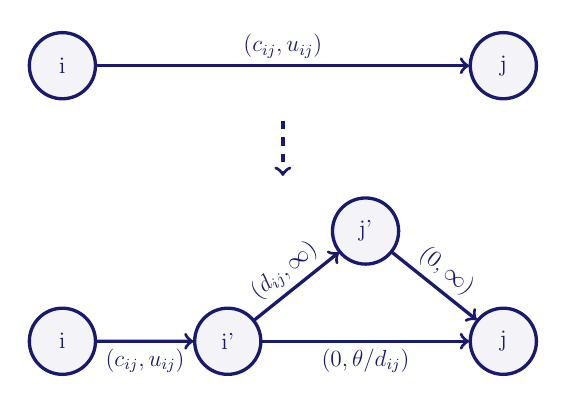
\begin{tikzpicture}[scale=0.7, every node/.style={transform shape},
roundnode/.style={circle, draw=MidnightBlue, fill=MidnightBlue!5, very thick, minimum size=12mm}]
\tikzset{myline/.style={very thick, draw=MidnightBlue,->}}
%Nodes
\node at (0,0) [roundnode] (I)	{\color{MidnightBlue}\large{i}};
\node at (8,0) [roundnode] (J)	{\color{MidnightBlue}\large{j}};

\draw[very thick, dashed, MidnightBlue,->]	(4,-1) -- (4,-2);

\node at (0,-5) 	[roundnode] (I2)	{\color{MidnightBlue}\large{i}};
\node at (8,-5) 	[roundnode] (J2)	{\color{MidnightBlue}\large{j}};
\node at (3,-5)		[roundnode] (I')	{\color{MidnightBlue}\large{i'}};
\node at (5.5,-3)	[roundnode] (J')	{\color{MidnightBlue}\large{j'}};
%Lines
\draw[myline] (I) -- node[above] {\color{MidnightBlue}\large{$(c_{ij},u_{ij})$}}	(J) ;
\draw[myline] (I2) -- node[below]{\color{MidnightBlue}\large{$(c_{ij},u_{ij})$}}	(I');
\draw[myline] (I') -- node[above,sloped] {\color{MidnightBlue}\large{$(d_{ij},\infty)$}}(J');
\draw[myline] (I') -- node[below] {\color{MidnightBlue}\large{$(0,\theta/d_{ij})$}}(J2);
\draw[myline] (J') -- node[above,sloped] {\color{MidnightBlue}\large{$(0,\infty)$}}(J2);
\end{tikzpicture}
\caption{Construction of $G'$}\label{ABB:bogen}
\end{figure}
Now we show that solving a Min Cost Flow problem on $G'$ leads to the solution of problem (\eqref{EQ:25}) 

Let $x*$ be an optimal solution to \eqref{EQ:25}. For every arc $(i,j)\in \mathcal{A}$, we consider two cases:
\begin{itemize}
	\item If $x^*_{ij}\leq\theta/d_{ij}$, then the flow $x^*_{ij}$will, in $G'$, flow via $(i,i')$ and $(i',j)$, leading to a cost of \[c_{ii'}x^*_{ij}+c_{i'j}x^*_{ij} = c_{ij}x^*_{ij}\].
	\item If $x^*_{ij}\geq\theta/d_{ij}$, then $x^*_{ij}$ is divided at node $i'$: A quanityt of $\theta/d_{ij}$ flows via $(i',j)$, while the excess $x^*_{ij}-(\theta/d_{ij})$ is routed via $(i',j')$ and $(j',j)$, such that the cost adds up to \[c_{ij}x_{ij}+d_{ij}\left(x_{ij}-\frac{\theta}{d_{ij}}\right).\]
\end{itemize}
In both cases, the contribution to cost matches the objective function value in \eqref{EQ:25}.
\end{proof}

It is straightforward to show that $Z(\theta)$ is a convex function. Thus, by executing a line search, we may approximate the optimal solution of \eqref{p3c4:solvedprob} to any degree of accuracy by executing a corresponding number of function evaluations, that is, min cost flow problems.